% ============================================================
%  LLM-as-a-Judge: Czy modele językowe nadają się na stanowisko
%  rekrutera technicznego?
%  Raport badawczy — Inteligencja Obliczeniowa, UG 2025/26
% ============================================================
\documentclass[12pt, a4paper]{article}

% --- Język i kodowanie ---
\usepackage[T1]{fontenc}
\usepackage[utf8]{inputenc}
\usepackage[polish]{babel}

% --- Marginesy ---
\usepackage[top=2.5cm, bottom=2.5cm, left=3cm, right=2.5cm]{geometry}

% --- Typografia ---
\usepackage{lmodern}
\usepackage{microtype}
\usepackage{setspace}
\onehalfspacing

% --- Tabele ---
\usepackage{booktabs}
\usepackage{multirow}
\usepackage{array}
\usepackage{xcolor}
\usepackage{colortbl}

% --- Grafika ---
\usepackage{graphicx}
\usepackage{float}

% --- Matematyka ---
\usepackage{amsmath}

% --- Kod źródłowy ---
\usepackage{listings}
\lstset{
    basicstyle=\ttfamily\small,
    breaklines=true,
    frame=single,
    backgroundcolor=\color{gray!10},
    keywordstyle=\color{blue},
    commentstyle=\color{green!50!black},
    stringstyle=\color{red!70!black},
    numbers=left,
    numberstyle=\tiny\color{gray},
    numbersep=5pt
}

% --- Hiperłącza ---
\usepackage[
    colorlinks=true,
    linkcolor=black,
    citecolor=blue!70!black,
    urlcolor=blue!70!black
]{hyperref}

% --- Bibliografia ---
\usepackage[
    backend=biber,
    style=numeric,
    sorting=none
]{biblatex}
\addbibresource{bibliografia.bib}

% --- Nagłówki sekcji ---
\usepackage{titlesec}
\titleformat{\section}{\large\bfseries}{\thesection.}{0.5em}{}
\titleformat{\subsection}{\normalsize\bfseries}{\thesubsection.}{0.5em}{}

% --- Definicje kolorów dla tabel ---
\definecolor{headerblue}{RGB}{52, 90, 140}
\definecolor{rowgray}{RGB}{240, 240, 240}

% ============================================================
\begin{document}

% ============================================================
%  STRONA TYTUŁOWA
% ============================================================
\begin{titlepage}
    \begin{center}
        \vspace*{1cm}
        {\Large\bfseries Uniwersytet Gdański\\
        Instytut Informatyki\\[0.3cm]}
        {\normalsize Inteligencja Obliczeniowa — rok akademicki 2025/2026\\[2cm]}

        \rule{\linewidth}{0.5mm}\\[0.4cm]
        {\LARGE\bfseries LLM-as-a-Judge:\\[0.3cm]
        Czy modele językowe nadają się\\
        na stanowisko rekrutera technicznego?}\\[0.4cm]
        \rule{\linewidth}{0.5mm}\\[2cm]

        {\large Raport badawczy}\\[3cm]

        % Dane autora idealnie wycentrowane na środku strony
        \begin{tabular}{ll}
            \textbf{Autor:}          & Jakub Jurkian \\[0.3cm]
            \textbf{Numer indeksu:}  & 300806 \\[0.3cm]
            \textbf{Prowadzący:}     & dr Grzegorz Madejski \\[0.3cm]
            \textbf{Data:}           & \today \\
        \end{tabular}
    \end{center}

    \vfill
\end{titlepage}

% ============================================================
%  SPIS TREŚCI
% ============================================================
\tableofcontents
\newpage

% ============================================================
%  1. WSTĘP
% ============================================================
\section{Wstęp}

Rekrutacja techniczna jest jednym z najbardziej czasochłonnych etapów w procesie zatrudnienia
programistów. Ocena kandydatów wymaga nie tylko czasu rekrutera, ale przede wszystkim
wiedzy eksperckiej pozwalającej zweryfikować poprawność udzielanych odpowiedzi.
Pojawia się więc naturalne pytanie: czy duże modele językowe (ang. \textit{Large Language Models},
LLM) mogłyby wspomóc lub zastąpić człowieka w tej roli?

Niniejszy raport bada paradygmat znany w literaturze jako \textit{LLM-as-a-Judge}
\cite{zheng2023judging} — zastosowanie modelu językowego jako automatycznego sędziego
oceniającego jakość odpowiedzi innego systemu lub człowieka.
W ramach projektu zbudowano system oceniający odpowiedzi kandydatów na stanowisko
Junior Java Developer, a następnie przeprowadzono serię eksperymentów porównujących
trzy modele językowe z dwóch różnych rodzin: lokalny model open-source oraz modele
komercyjne udostępniane przez API.

\subsection{Cel i pytania badawcze}

Głównym celem projektu jest ocena przydatności modeli językowych do automatycznej
ewaluacji odpowiedzi technicznych. W szczególności postawiono następujące pytania badawcze:

\begin{enumerate}
    \item Czy modele językowe potrafią rzetelnie oceniać odpowiedzi z zakresu
          programowania w Javie?
    \item Czy zastosowanie techniki RAG (\textit{Retrieval-Augmented Generation})
          poprawia jakość oceny w porównaniu z podejściem \textit{Pure Prompt}?
    \item Czy istnieją istotne różnice w jakości oceny między modelami z różnych
          rodzin (lokalny vs.\ komercyjny)?
\end{enumerate}

% ============================================================
%  2. PRZEGLĄD LITERATURY
% ============================================================
\section{Przegląd literatury}

\subsection{LLM-as-a-Judge}

Paradygmat \textit{LLM-as-a-Judge} został szeroko przebadany przez Zheng et al.\ \cite{zheng2023judging},
którzy zaproponowali platformę MT-Bench do oceny modeli językowych przy użyciu silniejszego
modelu jako sędziego. Autorzy wykazali, że modele GPT-4 jako sędziowie osiągają wysoką
zgodność z ocenami ekspertów ludzkich, jednak zidentyfikowali również szereg tendencji
(ang.\ \textit{biases}), takich jak preferowanie dłuższych odpowiedzi czy błędy pozycyjne.
Liu et al.\ \cite{liu2023geval} rozwinęli ten kierunek proponując G-Eval — metodę
oceny przy użyciu GPT-4 z dodatkowym łańcuchem rozumowania (\textit{chain-of-thought}),
osiągając jeszcze wyższą zgodność z ocenami ludzkimi w zadaniach generacji tekstu.
Z kolei Wang et al.\ \cite{wang2023fair} pokazują, że LLM-y jako sędziowie nie są
neutralne — wykazują istotny \textit{position bias} oraz preferują odpowiedzi
o określonej długości lub stylu. Aktualny przegląd literatury w tym obszarze
przedstawiają Li et al.\ \cite{li2024llmeval}, systematyzując otwarte problemy
metodyczne LLM-as-a-Judge.
Wyniki niniejszego projektu potwierdzają inny zidentyfikowany bias — tendencję
małych modeli do nadmiernej łagodności w ocenianiu (\textit{leniency bias}).

\subsection{Retrieval-Augmented Generation}

Technika RAG, zaproponowana przez Lewis et al.\ \cite{lewis2020rag}, polega na wzbogacaniu
promptu modelu o dokumenty pobrane z zewnętrznej bazy wiedzy na podstawie podobieństwa
semantycznego. Standardowe założenie jest takie, że dodatkowy kontekst poprawia jakość
odpowiedzi modelu. Aktualny przegląd ekosystemu RAG (architektury naive/advanced/modular,
strategie chunkowania, re-ranking) podają Gao et al.\ \cite{gao2024ragsurvey}.
Kluczowym komponentem retrievera są gęste reprezentacje wektorowe pytań i dokumentów;
Karpukhin et al.\ \cite{karpukhin2020dpr} wykazali w \textit{Dense Passage Retrieval},
że dwuwieżowy encoder trenowany kontrastywnie istotnie przewyższa BM25 w zadaniach QA.
Na poziomie infrastruktury, warstwa wyszukiwania w niniejszym projekcie (pgvector)
opiera się na algorytmie HNSW \cite{malkov2020hnsw}, który zapewnia logarytmiczną
złożoność wyszukiwania przybliżonego najbliższego sąsiada.

W kontekście ewaluacji jakości odpowiedzi, RAG może dostarczyć modelowi wzorcową odpowiedź,
względem której ocenia kandydata. Niemniej, jak wykazano w niniejszym badaniu,
dla domen dobrze pokrytych przez pre-training modeli (takich jak podstawy języka Java),
dodatkowy kontekst może wprowadzać zakłócenia zamiast poprawiać jakość oceny.

\subsection{Ewaluacja systemów RAG}

Framework RAGAS \cite{es2023ragas} dostarcza metodologię automatycznej ewaluacji
systemów RAG, oceniając między innymi wierność generowanych odpowiedzi
i trafność pobranych dokumentów. Niniejszy projekt przyjmuje odmienną perspektywę —
zamiast ewaluować system RAG pod kątem generowania odpowiedzi, bada wpływ RAG
na jakość oceny dokonywanej przez model-sędziego.

% ============================================================
%  3. ARCHITEKTURA SYSTEMU
% ============================================================
\section{Architektura systemu}

\subsection{Stos technologiczny}

System MockBean został zbudowany w oparciu o następujące technologie:

\begin{itemize}
    \item \textbf{Java 21 + Spring Boot 3.5} — warstwa backendowa z REST API
    \item \textbf{LangChain4j 0.29.1} — integracja z modelami językowymi
    \item \textbf{PostgreSQL + pgvector} — baza wektorowa do przechowywania embeddingów
    \item \textbf{Ollama} — lokalne uruchamianie modelu open-source
    \item \textbf{Python} — skrypt ewaluacyjny do automatycznego testowania
\end{itemize}

\subsection{Przepływ danych}

Rysunek~\ref{fig:architecture} przedstawia architekturę systemu. Dla trybu RAG
przepływ wygląda następująco:

\begin{enumerate}
    \item Pytanie rekrutacyjne jest konwertowane na wektor przez model embeddingowy
          (\texttt{nomic-embed-text})
    \item Pgvector wyszukuje najbardziej podobną wzorcową odpowiedź (top-1)
    \item Model-sędzia otrzymuje pytanie, wzorcową odpowiedź i odpowiedź kandydata
    \item Model zwraca ocenę w formacie JSON: wynik liczbowy, mocne strony,
          pominięte koncepcje i feedback tekstowy
\end{enumerate}

W trybie \textit{Pure Prompt} krok 1 i 2 są pomijane — model ocenia wyłącznie
na podstawie własnej wiedzy z pre-trainingu.

\begin{figure}[H]
    \centering
    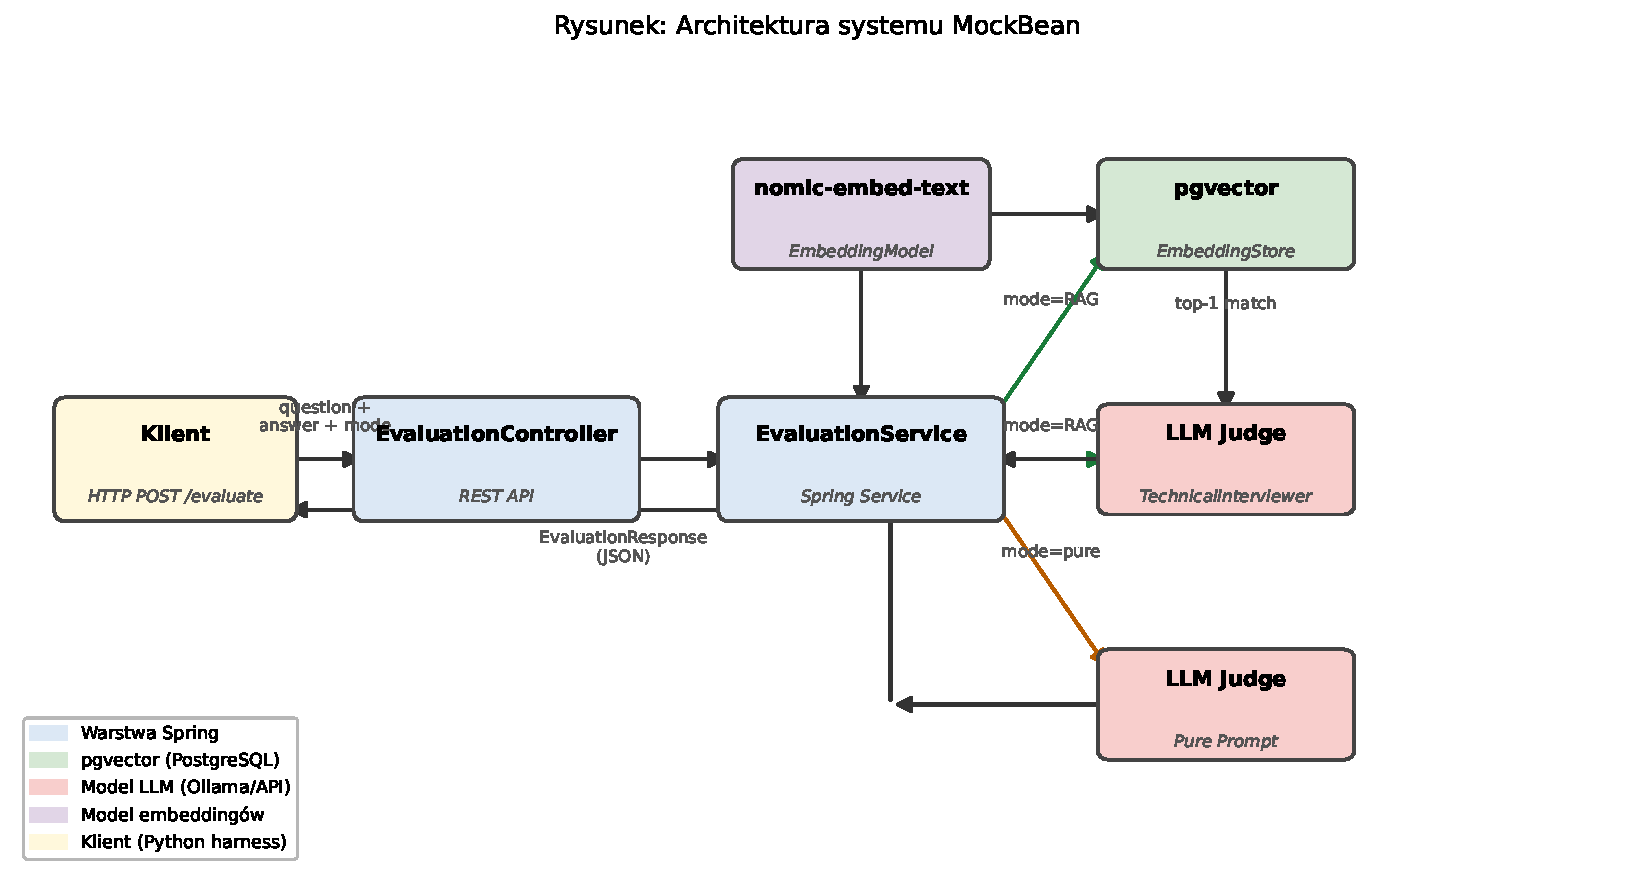
\includegraphics[width=0.92\textwidth]{architektura.pdf}
    \caption{Architektura systemu MockBean}
    \label{fig:architecture}
\end{figure}

\subsection{Przełączanie modeli}

Dzięki mechanizmowi profili Spring Boot możliwe jest uruchomienie aplikacji z dowolnym
z trzech modeli bez modyfikacji kodu. Każdy profil ładuje odrębny plik konfiguracyjny
YAML definiujący endpoint i klucz API odpowiedniego dostawcy.
Klasa konfiguracyjna oznaczona adnotacją \texttt{@Primary} zapewnia, że Spring wstrzykuje
właściwy bean \texttt{ChatLanguageModel} do warstwy serwisowej.

% ============================================================
%  4. METODOLOGIA
% ============================================================
\section{Metodologia}

\subsection{Zestaw testowy}

Na potrzeby badania stworzono ręcznie zestaw 40 par pytanie–odpowiedź z zakresu
Core Java i programowania obiektowego (OOP). Każda para została opatrzona etykietą
ludzką należącą do jednej z pięciu klas, po 8 przypadków na klasę
(tabela~\ref{tab:labels}).

\begin{table}[H]
    \centering
    \caption{Klasy etykiet w zestawie testowym}
    \label{tab:labels}
    \begin{tabular}{@{}lll@{}}
        \toprule
        \textbf{Etykieta} & \textbf{Opis} & \textbf{Liczba} \\
        \midrule
        \texttt{correct}  & Odpowiedź poprawna i wyczerpująca & 8 \\
        \texttt{partial}  & Odpowiedź częściowo poprawna, brakuje głębi & 8 \\
        \texttt{wrong}    & Odpowiedź zawiera błędy merytoryczne & 8 \\
        \texttt{waffle}   & Odpowiedź brzmi mądrze, ale jest merytorycznie pusta & 8 \\
        \texttt{evasive}  & Odpowiedź unikająca, kandydat przyznaje się do niewiedzy & 8 \\
        \midrule
        \textbf{Łącznie}  & & \textbf{40} \\
        \bottomrule
    \end{tabular}
\end{table}

Klasy \texttt{wrong}, \texttt{waffle} i \texttt{evasive} tworzą grupę
\textit{adversarialną} — odpowiedzi które nie zasługują na pozytywną ocenę,
ale mogą zmylić model-sędziego.

\subsection{Badane modele}

W eksperymencie porównano trzy modele językowe z różnych rodzin
(tabela~\ref{tab:models}).

\begin{table}[H]
    \centering
    \caption{Badane modele językowe}
    \label{tab:models}
    \begin{tabular}{@{}llll@{}}
        \toprule
        \textbf{Model} & \textbf{Dostawca} & \textbf{Typ} & \textbf{Parametry} \\
        \midrule
        llama3.1:8b        & Meta (Ollama) & Lokalny, open-source & 8B  \\
        claude-sonnet-4-6  & Anthropic     & Komercyjny, API      & n/d \\
        gemini-2.5-flash   & Google        & Komercyjny, API      & n/d \\
        \bottomrule
    \end{tabular}
\end{table}

\subsection{Tryby ewaluacji}

Każdy model przetestowano w dwóch trybach:

\begin{itemize}
    \item \textbf{RAG} — model otrzymuje wzorcową odpowiedź pobraną z bazy wektorowej
          pgvector (top-1 similarity search na embeddingach \texttt{nomic-embed-text})
    \item \textbf{Pure Prompt} — model ocenia wyłącznie na podstawie własnej wiedzy,
          bez dostarczonego kontekstu
\end{itemize}

\subsection{Metryki}

\paragraph{Mapowanie ocen na klasy.}
Model-sędzia zwraca wynik liczbowy $s \in [0, 1]$.
Zastosowano następujące progi klasyfikacyjne:

\begin{align}
    \hat{y} = \begin{cases}
        \texttt{correct} & \text{jeśli } s \geq 0{,}65 \\
        \texttt{partial} & \text{jeśli } 0{,}30 \leq s < 0{,}65 \\
        \texttt{low}     & \text{jeśli } s < 0{,}30
    \end{cases}
\end{align}

Etykiety ludzkie \texttt{wrong}, \texttt{waffle} i \texttt{evasive}
są mapowane na klasę \texttt{low}.

\paragraph{Accuracy.}
Główna metryka: odsetek przypadków gdzie przewidziana klasa zgadza się z etykietą ludzką.

\paragraph{Gullibility.}\label{sec:metrics-gull}
Odsetek odpowiedzi \texttt{waffle} i \texttt{evasive} którym model przyznał
wynik $s \geq 0{,}5$ — miara podatności na manipulację.
Pełne wyniki dla wszystkich konfiguracji podaje sekcja~\ref{sec:gullibility}.

\paragraph{Stabilność.}
Każdy eksperyment powtórzono dwukrotnie przy \texttt{temperature=0.0}.
Różnica accuracy między runami $|\Delta| \leq 2{,}5\%$ uznawana jest za stabilną.

% ============================================================
%  5. WYNIKI
% ============================================================
\section{Wyniki}

\subsection{Accuracy — zestawienie główne}

Tabela~\ref{tab:main_results} przedstawia wyniki accuracy dla wszystkich kombinacji
modelu i trybu ewaluacji.

\begin{table}[H]
    \centering
    \caption{Accuracy (\%) — wszystkie modele i tryby}
    \label{tab:main_results}
    \begin{tabular}{@{}lcccc@{}}
        \toprule
        \multirow{2}{*}{\textbf{Model}}
            & \multicolumn{2}{c}{\textbf{RAG}}
            & \multicolumn{2}{c}{\textbf{Pure Prompt}} \\
        \cmidrule(lr){2-3} \cmidrule(lr){4-5}
            & Run 1 & Run 2 & Run 1 & Run 2 \\
        \midrule
        llama3.1:8b       & 50,0\% & 50,0\% & 57,5\% & 57,5\% \\
        gemini-2.5-flash  & 80,0\% & 80,0\% & 87,5\% & 82,5\% \\
        claude-sonnet-4-6 & 82,5\% & 82,5\% & 92,5\% & 92,5\% \\
        \bottomrule
    \end{tabular}
\end{table}

\subsection{Baseline non-LLM: TF-IDF + cosine similarity}
\label{sec:baseline}

Aby umieścić wyniki modeli językowych na tle klasycznej techniki analizy tekstu,
zaimplementowano w czystym Pythonie baseline oparty na reprezentacji
\textit{bag of words} z wagami TF-IDF oraz miarą cosine similarity
\cite{karpukhin2020dpr}. Pipeline replikuje strukturę trybu RAG modeli LLM,
zapewniając porównywalność:

\begin{enumerate}
    \item Retrieval: dla pytania testowego wybierany jest najbardziej
          podobny wzorzec z bazy wiedzy (TF-IDF cosine między pytaniami).
    \item Scoring: liczone jest cosine similarity między wektorem
          TF-IDF odpowiedzi kandydata a wektorem TF-IDF wzorcowej
          odpowiedzi z pobranego rekordu.
    \item Mapowanie: wynik traktowany jest jak \texttt{score} modelu-sędziego
          i mapowany na bucket tymi samymi progami (0,65 / 0,30).
\end{enumerate}

Baseline jest deterministyczny, darmowy (latencja $<10$ ms per zapytanie)
i całkowicie pozbawiony rozumienia semantycznego — sygnałem jest wyłącznie
leksykalna zbieżność słów. Wyniki zestawia tabela~\ref{tab:baseline}
i wizualizuje rysunek~\ref{fig:baseline_comparison}.

\begin{table}[H]
    \centering
    \caption{TF-IDF + cosine baseline vs.\ modele LLM w trybie Pure (accuracy per etykieta)}
    \label{tab:baseline}
    \begin{tabular}{@{}lcccccc@{}}
        \toprule
        \textbf{System} & \textbf{correct} & \textbf{partial}
            & \textbf{wrong} & \textbf{waffle}
            & \textbf{evasive} & \textbf{Overall} \\
        \midrule
        TF-IDF baseline    & 62\%  & \textbf{100\%} & \textbf{0\%}   & 75\%  & 62\%  & 60,0\% \\
        \midrule
        llama · Pure       & 100\% & 62\%  & 25\%  & 62\%  & 38\%  & 57,5\% \\
        gemini · Pure      & 88\%  & 88\%  & 88\%  & 88\%  & 88\%  & 85,0\% \\
        claude · Pure      & 88\%  & 100\% & 88\%  & 88\%  & 100\% & 92,5\% \\
        \bottomrule
    \end{tabular}
\end{table}

\begin{figure}[H]
    \centering
    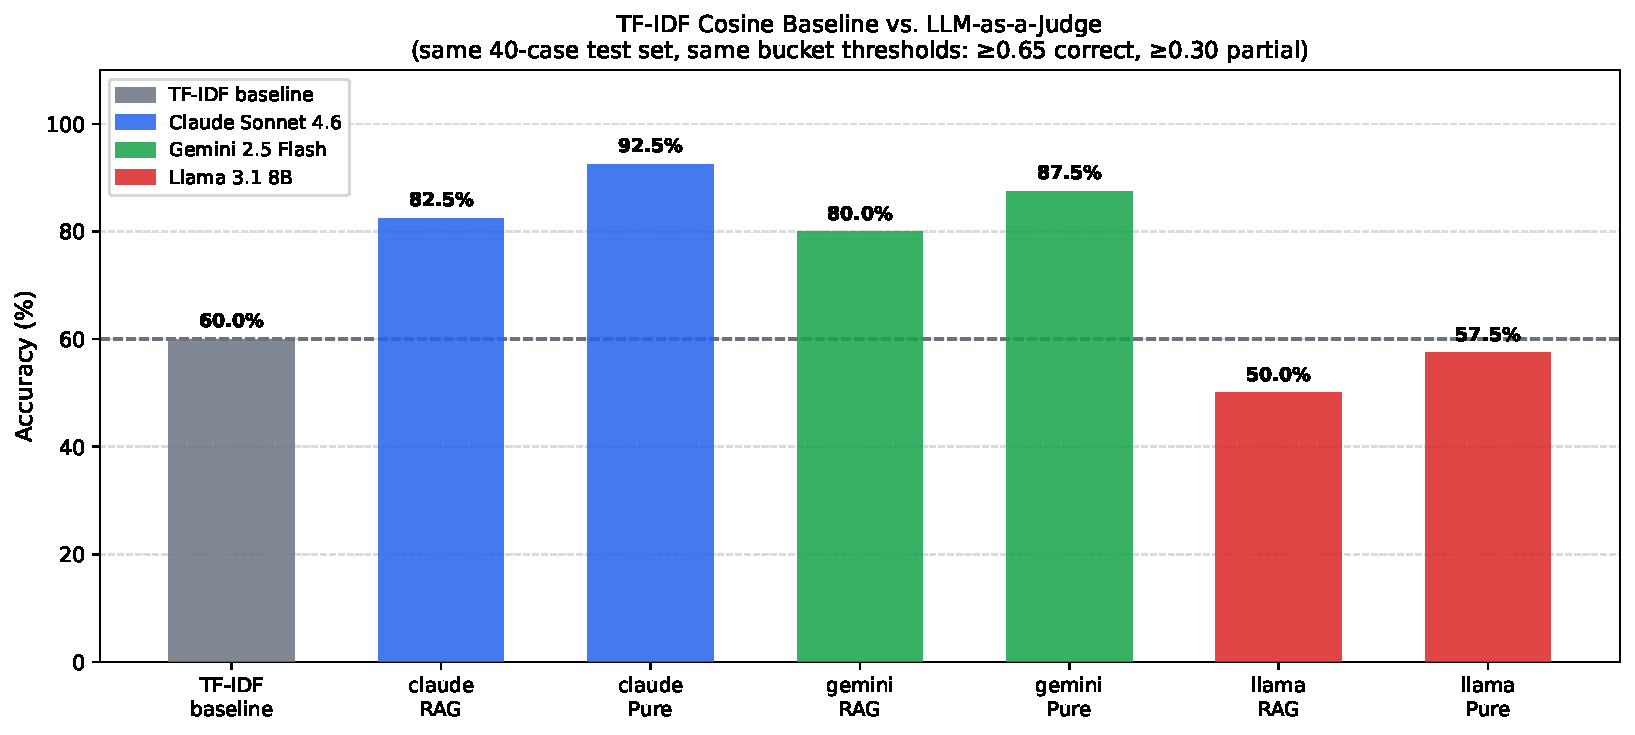
\includegraphics[width=0.92\textwidth]{fig_baseline_comparison.pdf}
    \caption{Porównanie accuracy: baseline TF-IDF cosinus vs.\ wszystkie eksperymenty LLM-as-a-Judge.
             Przerywana linia oznacza poziom baseline (60,0\%).}
    \label{fig:baseline_comparison}
\end{figure}

Baseline osiągnął 60,0\% overall accuracy, co minimalnie przewyższa
\texttt{llama · Pure} (57,5\%) mimo że nie używa żadnego modelu deep
learning ani semantycznego rozumienia. Analiza per etykieta ujawnia
ciekawą strukturę podobieństwa leksykalnego względem semantycznego:

\begin{itemize}
    \item Na klasie \texttt{partial} baseline osiąga 100\% trafności —
          odpowiedzi częściowo poprawne są leksykalnie najbardziej zbliżone
          do wzorca (kandydat używa tych samych terminów, ale brakuje
          mu głębi), więc trafiają dokładnie w przedział
          $0{,}30 \leq s < 0{,}65$ odpowiadający bucketowi \texttt{partial}.
    \item Na klasie \texttt{wrong} baseline kompletnie zawodzi (0\%) —
          błędne odpowiedzi techniczne często używają tych samych
          terminów co poprawne (np.\ \textit{garbage collector},
          \textit{synchronized}, \textit{stream}), więc dostają wysokie
          podobieństwo TF-IDF i są klasyfikowane jako \texttt{correct}
          lub \texttt{partial}, mimo że są merytorycznie błędne.
          LLM rozróżnia znaczenia; TF-IDF nie.
    \item Na klasach \texttt{waffle} (75\%) i \texttt{evasive} (62\%)
          baseline radzi sobie umiarkowanie dobrze — odpowiedzi puste
          lub uchylne mają mniejsze pokrycie słownikowe z wzorcem
          i częściej spadają w bucket \texttt{low}, ale nie zawsze
          (część odpowiedzi \texttt{waffle} przemyca dość terminów
          technicznych, by przekroczyć próg 0,30).
    \item Na klasie \texttt{correct} (62\%) baseline trafia tylko
          część poprawnych odpowiedzi — kandydaci używają synonimów
          i innej struktury zdań niż wzorzec, co obniża podobieństwo
          leksykalne poniżej progu 0,65.
\end{itemize}

Najlepszy model LLM (\texttt{claude-sonnet-4-6}, tryb Pure Prompt) uzyskuje
92,5\%, co daje \textbf{przewagę $+32{,}5$~pp} nad baseline'em i potwierdza,
że modele językowe wnoszą realną wartość dodaną — potrafią oceniać
merytoryczną poprawność odpowiedzi, a nie tylko powierzchowne podobieństwo
słowne. Wyjątkiem pozostaje \texttt{llama · RAG}, która przy accuracy 50\%
nieznacznie wyprzedza random baseline ($\frac{1}{3} \approx 33{,}3\%$
przy trójklasowej klasyfikacji) i wyraźnie ustępuje TF-IDF.

\paragraph{Wniosek pragmatyczny.}
W systemie produkcyjnym sensowna byłaby hybryda: szybki filtr TF-IDF
(latencja $<10$ ms, koszt zerowy) pozwala odrzucić znaczną część
oczywiście pustych odpowiedzi, a kosztowne wywołania LLM rezerwowane
są dla przypadków wątpliwych. Taki układ pozwala obniżyć koszty API
bez istotnej utraty trafności klasyfikacji.

\subsection{Accuracy per etykieta}

Tabela~\ref{tab:per_label} przedstawia dokładność klasyfikacji z podziałem
na poszczególne klasy (wartości uśrednione z dwóch runów; dla \texttt{gemini · Pure},
gdzie runy różnią się o 5~pp, wartości w kolumnie \textbf{Overall} są średnią
arytmetyczną Run~1 i Run~2, co daje 85,0\%).

\begin{table}[H]
    \centering
    \caption{Accuracy per etykieta (\%)}
    \label{tab:per_label}
    \begin{tabular}{@{}lcccccc@{}}
        \toprule
        \textbf{Model / Tryb}
            & \textbf{correct} & \textbf{partial}
            & \textbf{wrong}   & \textbf{waffle}
            & \textbf{evasive} & \textbf{Overall} \\
        \midrule
        llama · RAG        & 100\% & 25\% & 12\%  & 50\%  & 62\%  & 50,0\% \\
        llama · Pure       & 100\% & 62\% & 25\%  & 62\%  & 38\%  & 57,5\% \\
        \midrule
        gemini · RAG       & 88\%  & 62\% & 88\%  & 88\%  & 75\%  & 80,0\% \\
        gemini · Pure      & 82\%  & 82\% & 88\%  & 88\%  & 88\%  & 85,0\% \\
        \midrule
        claude · RAG       & 88\%  & 62\% & 88\%  & 88\%  & 88\%  & 82,5\% \\
        claude · Pure      & 88\%  & 100\%& 88\%  & 88\%  & 100\% & 92,5\% \\
        \bottomrule
    \end{tabular}
\end{table}

\subsection{Przedziały ufności (Bootstrap)}

Ze względu na ograniczony rozmiar zestawu testowego ($n = 40$) obliczono
bootstrapowe 95\% przedziały ufności dla accuracy każdego eksperymentu
($B = 10\,000$ prób, ziarno 42, próbkowanie ze zwracaniem).
Przedziały ufności w tabeli~\ref{tab:bootstrap_ci} liczone są na danych z~Run~1
każdego eksperymentu; dla pięciu z sześciu konfiguracji Run~2 daje identyczny
zestaw ocen (patrz tabela~\ref{tab:stability}), więc wynik bootstrapowy byłby
nieodróżnialny. Wyjątkiem jest \texttt{gemini · Pure}, gdzie $\Delta = 5$~pp
między runami — wartości w tabeli odnoszą się tu konkretnie do Run~1 (87,5\%).

\begin{table}[H]
    \centering
    \caption{Accuracy z bootstrapowym 95\% przedziałem ufności ($n=10\,000$ prób)}
    \label{tab:bootstrap_ci}
    \begin{tabular}{@{}lcccc@{}}
        \toprule
        \textbf{Eksperyment} & \textbf{Accuracy} & \textbf{CI dolny} & \textbf{CI górny} & \textbf{$\pm$half} \\
        \midrule
        claude · RAG         & 82,5\% & 70,0\% & 92,5\% & $\pm$11,2\% \\
        claude · Pure        & 92,5\% & 82,5\% & 100,0\% & $\pm$8,8\% \\
        gemini · RAG         & 80,0\% & 67,5\% & 92,5\% & $\pm$12,5\% \\
        gemini · Pure        & 87,5\% & 77,5\% & 97,5\% & $\pm$10,0\% \\
        llama · RAG          & 50,0\% & 35,0\% & 65,0\% & $\pm$15,0\% \\
        llama · Pure         & 57,5\% & 42,5\% & 72,5\% & $\pm$15,0\% \\
        \bottomrule
    \end{tabular}
\end{table}

\begin{figure}[H]
    \centering
    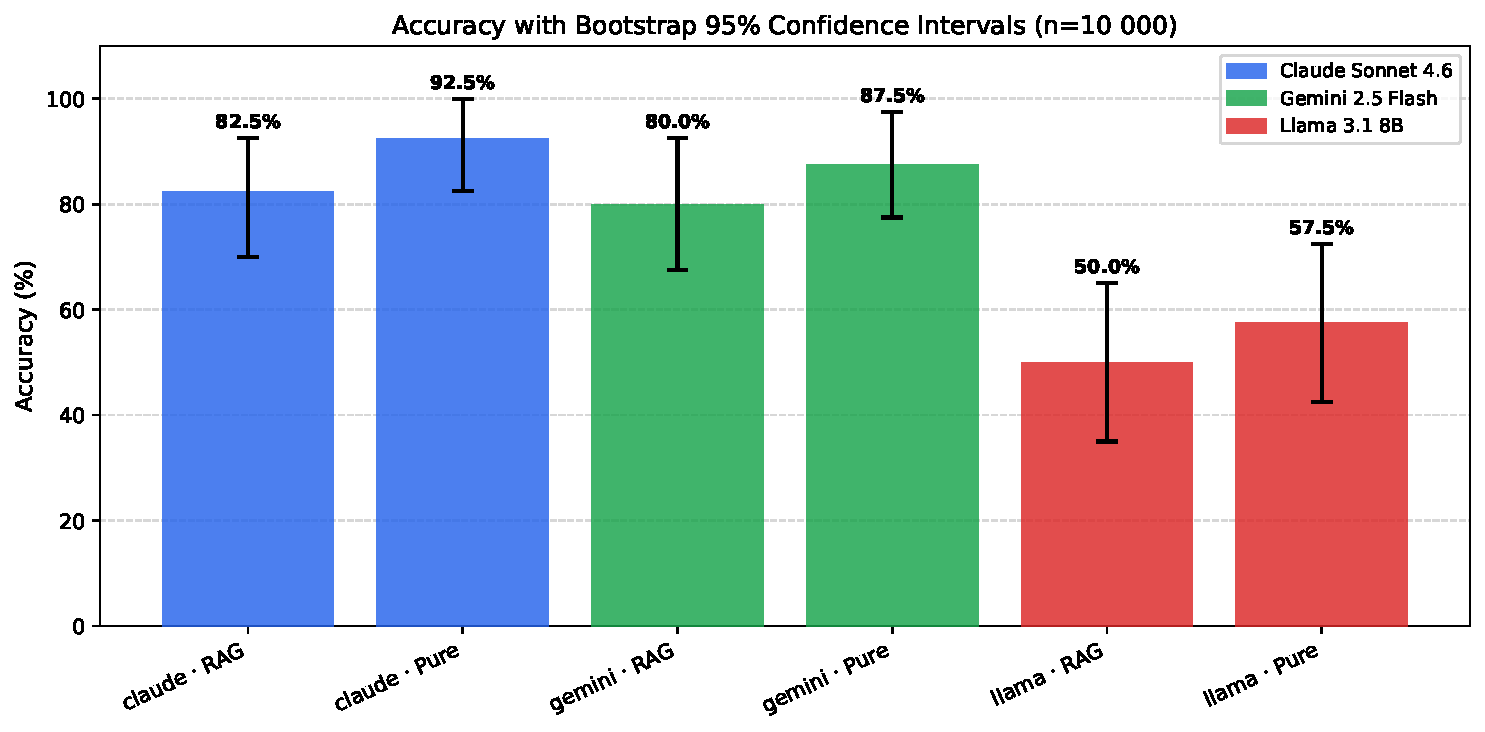
\includegraphics[width=0.90\textwidth]{fig_bootstrap_ci.pdf}
    \caption{Accuracy z bootstrapowymi 95\% przedziałami ufności dla wszystkich eksperymentów}
    \label{fig:bootstrap_ci}
\end{figure}

Szerokość przedziałów ($\pm 8{,}8$--$15{,}0$ pp) odzwierciedla ograniczony
rozmiar zestawu testowego i należy ją uwzględnić przy interpretacji wyników.
Mimo to claude · Pure konsekwentnie wyprzedza pozostałe eksperymenty, a
dolna granica jego CI (82,5\%) jest wyższa niż górna granica llama · Pure (72,5\%),
co wskazuje na statystycznie istotną różnicę między tymi dwoma modelami.

\subsection{Stabilność wyników}

\begin{table}[H]
    \centering
    \caption{Stabilność wyników — różnica między runami}
    \label{tab:stability}
    \begin{tabular}{@{}lcccl@{}}
        \toprule
        \textbf{Eksperyment} & \textbf{Run 1} & \textbf{Run 2}
            & \textbf{$|\Delta|$} & \textbf{Ocena} \\
        \midrule
        llama · RAG        & 50,0\% & 50,0\% & 0,0\% & Stabilny \\
        llama · Pure       & 57,5\% & 57,5\% & 0,0\% & Stabilny \\
        gemini · RAG       & 80,0\% & 80,0\% & 0,0\% & Stabilny \\
        gemini · Pure      & 87,5\% & 82,5\% & 5,0\% & Niestabilny \\
        claude · RAG       & 82,5\% & 82,5\% & 0,0\% & Stabilny \\
        claude · Pure      & 92,5\% & 92,5\% & 0,0\% & Stabilny \\
        \bottomrule
    \end{tabular}
\end{table}

\subsection{Latencja i koszt eksperymentu}

Z punktu widzenia wdrożenia produkcyjnego sama trafność nie wystarcza —
istotne są również czas odpowiedzi (od momentu wysłania żądania do otrzymania
oceny w JSON) oraz koszt jednej oceny. Tabela~\ref{tab:latency} podsumowuje
statystyki latencji obliczone na danych z Run~1 ($n=40$ wywołań).

\begin{table}[H]
    \centering
    \caption{Latencja end-to-end pojedynczej oceny (ms) — Run~1, $n=40$}
    \label{tab:latency}
    \begin{tabular}{@{}lrrrrl@{}}
        \toprule
        \textbf{Eksperyment}
            & \textbf{średnia} & \textbf{mediana}
            & \textbf{p95}     & \textbf{maks.}
            & \textbf{Rozliczenie} \\
        \midrule
        claude · RAG    &  6\,177 &  6\,138 &  8\,045 &  8\,711 & API (Anthropic) \\
        claude · Pure   &  7\,496 &  7\,474 &  9\,106 &  9\,558 & API (Anthropic) \\
        gemini · RAG    &  6\,256 &  5\,958 & 10\,119 & 11\,683 & API (Google)    \\
        gemini · Pure   &  6\,765 &  6\,804 &  8\,364 &  9\,183 & API (Google)    \\
        llama · RAG     & 23\,396 & 22\,162 & 35\,222 & 37\,163 & lokalnie (CPU)  \\
        llama · Pure    & 25\,649 & 25\,204 & 35\,913 & 45\,176 & lokalnie (CPU)  \\
        \bottomrule
    \end{tabular}
\end{table}

\paragraph{Łączny czas eksperymentu.}
Pełne odtworzenie pojedynczego runu (40 wywołań sekwencyjnych)
trwa: claude $\approx$ 4--5~min, gemini $\approx$ 4--4,5~min,
llama $\approx$ 15,5--17~min. Llama jest tu istotnie wolniejsza,
ponieważ działa lokalnie przez Ollama na CPU — z dostępem do GPU
różnica zmniejszyłaby się do akceptowalnego poziomu.

\paragraph{Koszt.}
Modele API rozliczane są od liczby tokenów wejściowych i wyjściowych.
Średnia długość promptu w trybie RAG to ok. 500--700 tokenów (system message
+ pytanie + wzorzec + odpowiedź kandydata), a odpowiedź JSON ok. 300--500
tokenów. Przyjmując publiczne stawki obowiązujące w momencie eksperymentów
(Claude Sonnet 4.6: 3~USD/1M input, 15~USD/1M output; Gemini 2.5 Flash:
0{,}30/2{,}50~USD analogicznie), koszt 40 ocen mieści się w okolicy:
$\sim$0,30~USD dla Claude i $\sim$0,03~USD dla Gemini.
Llama3.1:8b uruchamiana przez Ollama lokalnie jest darmowa
w sensie pieniężnym, ale generuje wyraźny koszt czasowy.

\paragraph{Trade-off.}
Zestawienie z tabelą~\ref{tab:main_results} pokazuje wyraźny pareto-front:
Claude osiąga najwyższą accuracy przy najwyższym koszcie pieniężnym,
Gemini daje niemal porównywalną trafność za jedną dziesiątą ceny,
a Llama jest opcją „darmową, ale niedokładną i wolną".
Dla scenariusza ewaluacyjnego, w którym jakość oceny przekłada się
bezpośrednio na decyzję rekrutacyjną, koszt API jest pomijalny
i wybór Claude jest uzasadniony.

\subsection{Gullibility — odporność na odpowiedzi adversarialne}
\label{sec:gullibility}

Metryka \textit{gullibility}, zdefiniowana w sekcji~\ref{sec:metrics-gull},
mierzy odsetek odpowiedzi z klas \texttt{waffle} (puste, ale brzmiące mądrze)
oraz \texttt{evasive} (uchylne, „nie wiem"), którym sędzia przyznał wynik
$s \geq 0{,}5$. Niska wartość świadczy o wysokiej odporności sędziego
na próby zmylenia. Zestawienie dla wszystkich siedmiu konfiguracji
(6 LLM-owych + baseline TF-IDF) podaje tabela~\ref{tab:gullibility}.

\begin{table}[H]
    \centering
    \caption{Gullibility ($\%$ odpowiedzi adversarialnych z $s \geq 0{,}5$, Run~1, $n_{adv}=16$)}
    \label{tab:gullibility}
    \begin{tabular}{@{}lcccl@{}}
        \toprule
        \textbf{System}
            & \textbf{waffle ($\geq 0{,}5$)}
            & \textbf{evasive ($\geq 0{,}5$)}
            & \textbf{gullibility} & \textbf{Komentarz} \\
        \midrule
        TF-IDF baseline    & 0/8 & 0/8 & 0,0\%  & ślepy na semantykę, odporny z założenia \\
        claude · RAG       & 0/8 & 0/8 & 0,0\%  & idealna selektywność \\
        claude · Pure      & 0/8 & 0/8 & 0,0\%  & idealna selektywność \\
        gemini · Pure      & 0/8 & 0/8 & 0,0\%  & odporny w trybie Pure \\
        llama · RAG        & 0/8 & 0/8 & 0,0\%  & artefakt rozkładu — patrz dyskusja \\
        gemini · RAG       & 0/8 & 1/8 & 6,2\%  & jedna evasive zmyliła sędziego \\
        llama · Pure       & 1/8 & 1/8 & 12,5\% & najsłabszy filtr semantyczny \\
        \bottomrule
    \end{tabular}
\end{table}

Modele komercyjne wykazują pełną odporność na adversarialne odpowiedzi.
Llama w trybie Pure przepuszcza 12,5\% takich przypadków — to spójne
z obserwowanym dla niej \textit{leniency bias} (sekcja~\ref{sec:leniency}).
Zerowa gullibility Llamy w trybie RAG jest artefaktem rozkładu ocen,
a nie rzeczywistą czujnością: model po prostu rzadko przyznaje wynik
powyżej 0{,}5 niezależnie od jakości odpowiedzi.

% ============================================================
%  6. ANALIZA I DYSKUSJA
% ============================================================
\section{Analiza i dyskusja}

\subsection{RAG vs.\ Pure Prompt}

Najważniejszym i najbardziej zaskakującym wynikiem badania jest fakt, że tryb
\textit{Pure Prompt} przewyższa tryb RAG dla każdego z trzech badanych modeli
(tabela~\ref{tab:main_results}).
Wzrost accuracy wynosi od $+7{,}5$ pp dla modeli llama i gemini, do $+10$ pp dla Claude.

Hipoteza wyjaśniająca to zjawisko jest następująca: baza wiedzy dostarcza wzorcową
odpowiedź pobraną metodą top-1 similarity search. Jeśli pobrany dokument nie jest
semantycznie idealnie dopasowany do pytania, model-sędzia otrzymuje mylący punkt
odniesienia i może nagradzać odpowiedzi za leksykalne podobieństwo do wzorca zamiast
oceniać merytoryczną poprawność. Nazywamy to zjawisko \textit{biasem partial match}.

W trybie \textit{Pure Prompt} model ocenia na podstawie własnej wiedzy z pre-trainingu
— dla zagadnień z zakresu podstaw języka Java, które są wyjątkowo dobrze pokryte
w danych treningowych dużych modeli, okazuje się to skuteczniejszą strategią.

Wynik ten jest jednak specyficzny dla badanej domeny i nie powinien być uogólniany
na domeny niszowe lub wymagające aktualnej wiedzy, gdzie RAG jest niezastąpiony.

\subsection{Porównanie modeli}

Wyniki wskazują na wyraźne różnice między modelami (rysunek~\ref{fig:accuracy_chart}):

\begin{itemize}
    \item \textbf{claude-sonnet-4-6} osiągnął najwyższą accuracy (92,5\% w trybie Pure),
          wykazując przy tym pełną stabilność ($\Delta = 0\%$)
    \item \textbf{gemini-2.5-flash} uzyskał zbliżone wyniki (85\% średnio w trybie Pure),
          jednak z pewną niestabilnością ($\Delta = 5\%$ między runami)
    \item \textbf{llama3.1:8b} wyraźnie odstaje od modeli komercyjnych nawet w najlepszym
          trybie (57,5\%), co wskazuje że rozmiar i jakość modelu mają kluczowe znaczenie
          dla zadania LLM-as-a-Judge
\end{itemize}

\begin{figure}[H]
    \centering
    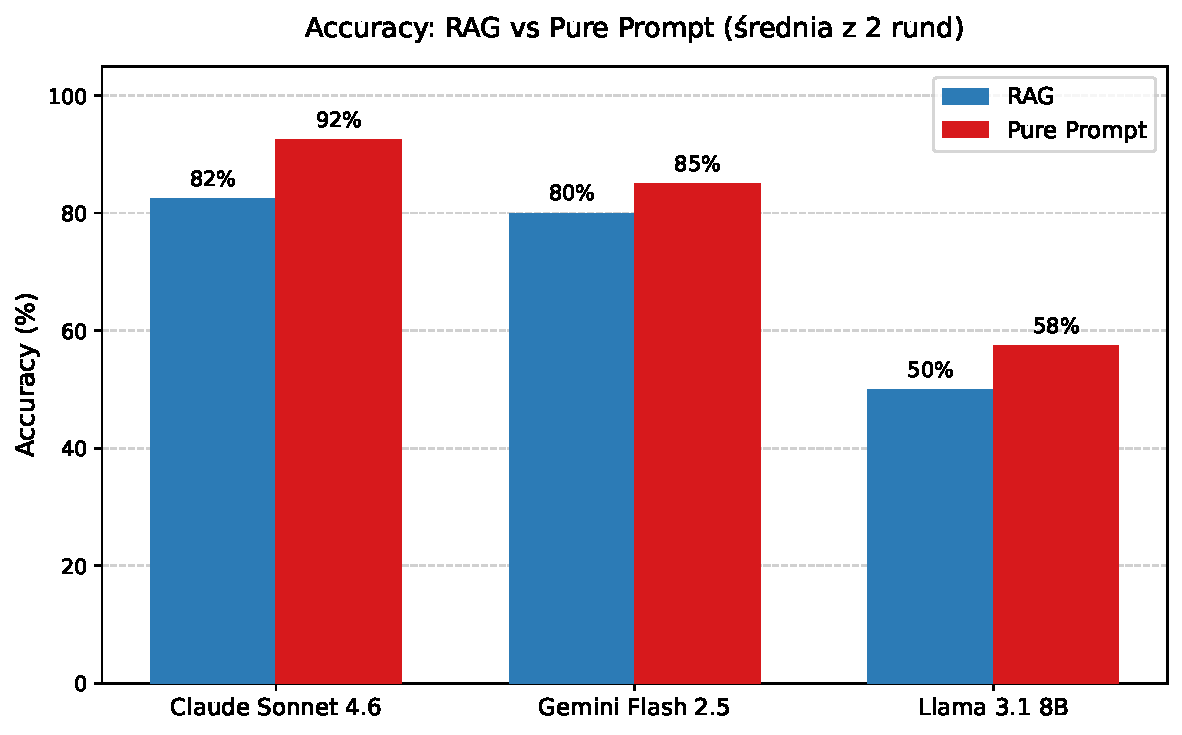
\includegraphics[width=0.88\textwidth]{fig_accuracy_comparison.pdf}
    \caption{Accuracy modeli w trybie RAG i Pure Prompt (średnia z 2 rund)}
    \label{fig:accuracy_chart}
\end{figure}

\begin{figure}[H]
    \centering
    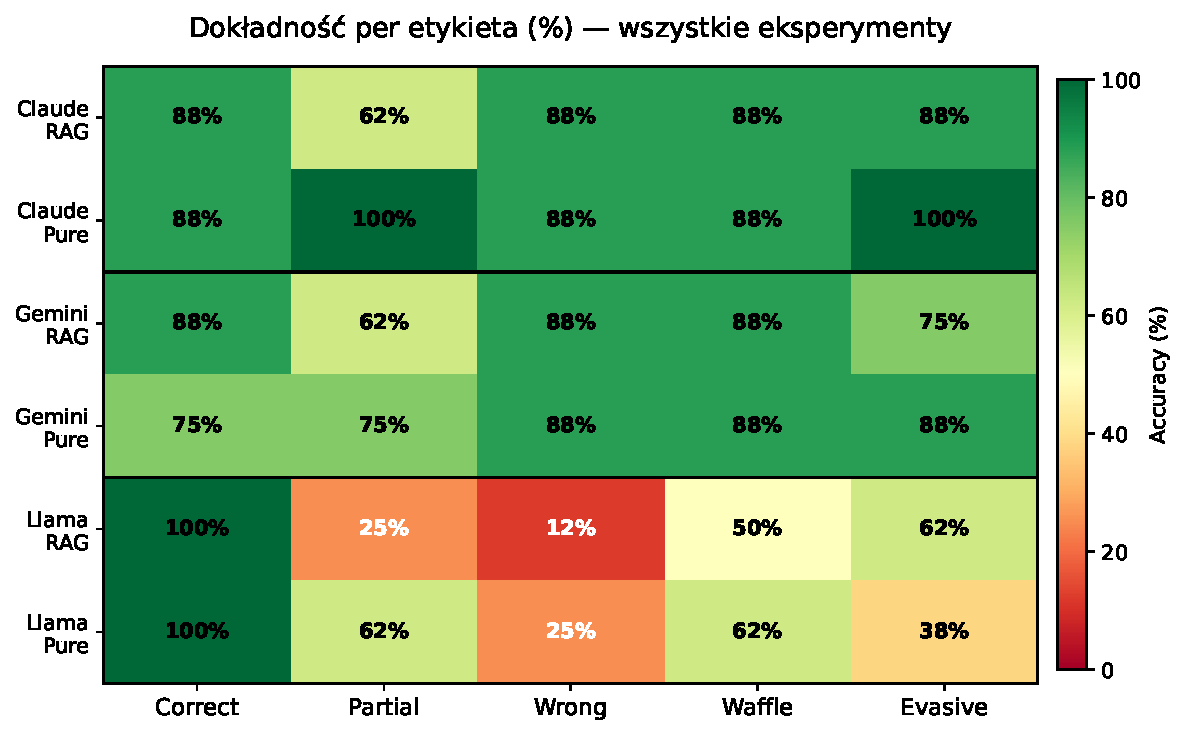
\includegraphics[width=0.88\textwidth]{fig_perlabel_heatmap.pdf}
    \caption{Dokładność per etykieta (\%) dla wszystkich kombinacji model~$\times$~tryb}
    \label{fig:perlabel_heatmap}
\end{figure}

Rysunek~\ref{fig:perlabel_heatmap} przedstawia szczegółowy rozkład dokładności
dla każdej etykiety i każdego eksperymentu. Widoczna jest wyraźna asymetria:
klasy \texttt{partial} oraz \texttt{wrong} sprawiają modelom największe trudności,
podczas gdy klasa \texttt{correct} jest rozpoznawana niemal bezbłędnie.

\subsection{Analiza biasu leniency}
\label{sec:leniency}

Llama3.1:8b w trybie RAG wykazuje szczególnie niską accuracy dla klasy \texttt{wrong}
(12\%) — model prawie nigdy nie wykrywa merytorycznie błędnych odpowiedzi.
Zjawisko to, znane w literaturze jako \textit{leniency bias} \cite{zheng2023judging},
polega na systematycznym zawyżaniu ocen przez model-sędziego.

Paradoksalnie, llama w trybie RAG osiąga 0\% gullibility (brak odpowiedzi
\texttt{waffle}/\texttt{evasive} z wynikiem $\geq 0{,}5$) — nie przez skuteczne
wykrywanie manipulacji, lecz dlatego że żadna odpowiedź nie przekroczyła progu 0{,}5,
co jest artefaktem rozkładu ocen, a nie rzeczywistą czujnością modelu.

\subsection{Niestabilność Gemini}

Przy ustawieniu \texttt{temperature=0.0}, llama i Claude wykazują pełną deterministyczność
($\Delta = 0\%$). Gemini-2.5-flash w trybie Pure Prompt wykazuje różnicę 5 pp między
runami, co wskazuje że Google nie gwarantuje pełnej powtarzalności wyników nawet
przy zerowej temperaturze — prawdopodobnie z powodu niedeterministycznej infrastruktury
serwerowej po stronie API. Jest to istotna uwaga praktyczna przy wdrożeniach
produkcyjnych systemów opartych na tym modelu.

% ============================================================
%  7. OGRANICZENIA
% ============================================================
\section{Ograniczenia badania}

\begin{enumerate}
    \item \textbf{Domena.} Badanie ogranicza się do zagadnień Core Java i OOP —
          dziedzin doskonale pokrytych przez pre-training dużych modeli.
          W domenach niszowych lub wymagających aktualnej wiedzy wyniki
          mogłyby być odmienne, a RAG mógłby okazać się korzystny.

    \item \textbf{Strategia retrieval.} Zastosowano top-1 similarity search.
          Podejście top-$k$ (np. $k=3$) mogłoby poprawić jakość RAG i zmienić
          wnioski dotyczące porównania trybów.

    \item \textbf{Rozmiar zestawu testowego.} 40 przypadków testowych pozwala
          wyciągać wstępne wnioski, jednak dla wyników statystycznie istotnych
          wymagany byłby większy zestaw danych.

    \item \textbf{Brak human baseline.} Progi klasyfikacyjne i etykiety ludzkie
          zostały wyznaczone przez autora bez walidacji przez niezależnych ekspertów.
          Nie przeprowadzono bezpośredniego porównania z ocenami prawdziwego rekrutera.

    \item \textbf{Kalibracja progów.} Zastosowane progi ($0{,}65$ i $0{,}30$)
          są stałe dla wszystkich modeli, mimo że rozkłady ocen różnią się
          między modelami (np.\ średnia ocena llamy to $0{,}517$, a Gemini $0{,}384$).
          Przeprowadzona analiza wrażliwości (rysunek~\ref{fig:threshold_sens})
          pokazuje, że najlepszy wynik (92,5\%) jest stabilny w szerokim zakresie
          progów dla Claude Pure, co potwierdza trafność wybranych wartości.
\end{enumerate}

\begin{figure}[H]
    \centering
    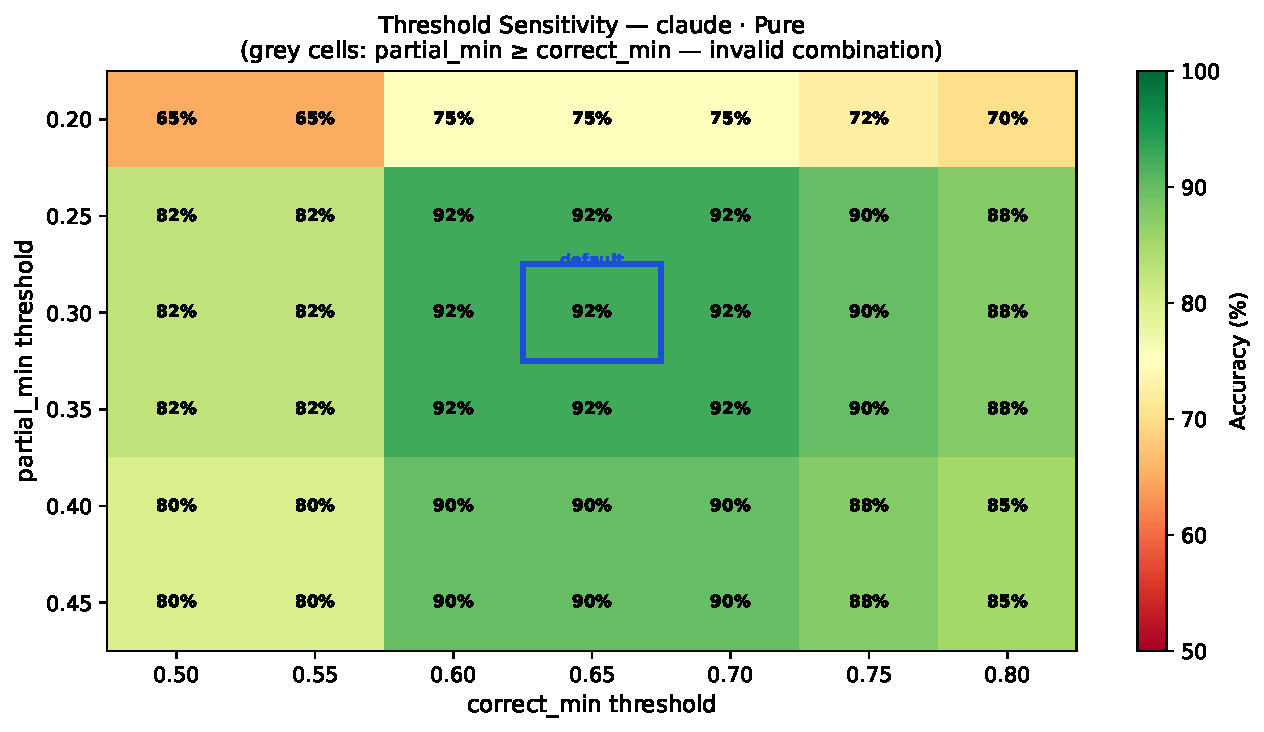
\includegraphics[width=0.88\textwidth]{fig_threshold_sens.pdf}
    \caption{Analiza wrażliwości progów klasyfikacyjnych dla eksperymentu claude~·~Pure.
             Niebieska ramka oznacza progi zastosowane w badaniu (0,65 / 0,30).
             Szare komórki to kombinacje niepoprawne ($\texttt{partial\_min} \geq \texttt{correct\_min}$).}
    \label{fig:threshold_sens}
\end{figure}

% ============================================================
%  8. WNIOSKI
% ============================================================
\section{Wnioski}

Niniejszy raport przedstawił wyniki badania oceniającego przydatność modeli językowych
do automatycznej ewaluacji odpowiedzi technicznych w kontekście rekrutacji na stanowisko
Junior Java Developer.

Najważniejsze wnioski są następujące:

\begin{enumerate}
    \item \textbf{Modele komercyjne są skutecznymi sędziami technicznymi.}
          Claude-sonnet-4-6 (92,5\%) i gemini-2.5-flash (85\%) osiągają wysoką accuracy,
          co czyni je obiecującymi narzędziami wspomagającymi rekrutację.

    \item \textbf{RAG jest kontrproduktywny dla dobrze znanych domen.}
          We wszystkich trzech badanych modelach tryb Pure Prompt przewyższa RAG,
          co sugeruje że dla zagadnień dobrze pokrytych przez pre-training,
          dodatkowy kontekst wprowadza bias partial match zamiast poprawiać ocenę.

    \item \textbf{Rozmiar modelu ma kluczowe znaczenie.}
          Llama3.1:8b, mimo że jest modelem open-source działającym lokalnie,
          pozostaje znacząco słabszym sędzią (57,5\%) niż modele komercyjne.
          Leniency bias sprawia, że model nagradza błędne odpowiedzi,
          co dyskwalifikuje go w roli autonomicznego sędziego rekrutacyjnego.

    \item \textbf{Deterministyczność jest ważna w zastosowaniach ewaluacyjnych.}
          Różnica w stabilności między Claude (pełny determinizm) a Gemini ($\Delta=5\%$)
          jest istotna praktycznie — powtarzalność wyników jest wymagana
          w rzetelnym procesie rekrutacyjnym.
\end{enumerate}

Odpowiadając na tytułowe pytanie: \textit{duże modele komercyjne} wykazują potencjał
jako narzędzie wspomagające rekrutera technicznego, jednak ze względu na zidentyfikowane
ograniczenia (brak human baseline, możliwy bias) powinny pełnić rolę uzupełniającą,
a nie zastępować ocenę eksperta.

Kierunkiem przyszłych badań mogłoby być porównanie ocen modeli z ocenami prawdziwych
rekruterów, co pozwoliłoby bezpośrednio odpowiedzieć na tytułowe pytanie.

% ============================================================
%  BIBLIOGRAFIA
% ============================================================
\printbibliography[title={Bibliografia}]

\end{document}
